%
% coord2d.tex
%
% (c) 2018 Prof Dr Andreas Müller, Hochschule Rapperswil
%
\documentclass[tikz]{standalone}
\usepackage{times}
\usepackage{amsmath}
\usepackage{txfonts}
\usepackage[utf8]{inputenc}
\usepackage{graphics}
\usepackage{color}
\usepackage{pifont}
\usetikzlibrary{arrows,intersections,math,calc}
\begin{document}

\def\punkt#1{
        \fill[color=white] #1 circle[radius=0.08];
        \draw #1 circle[radius=0.08];
}

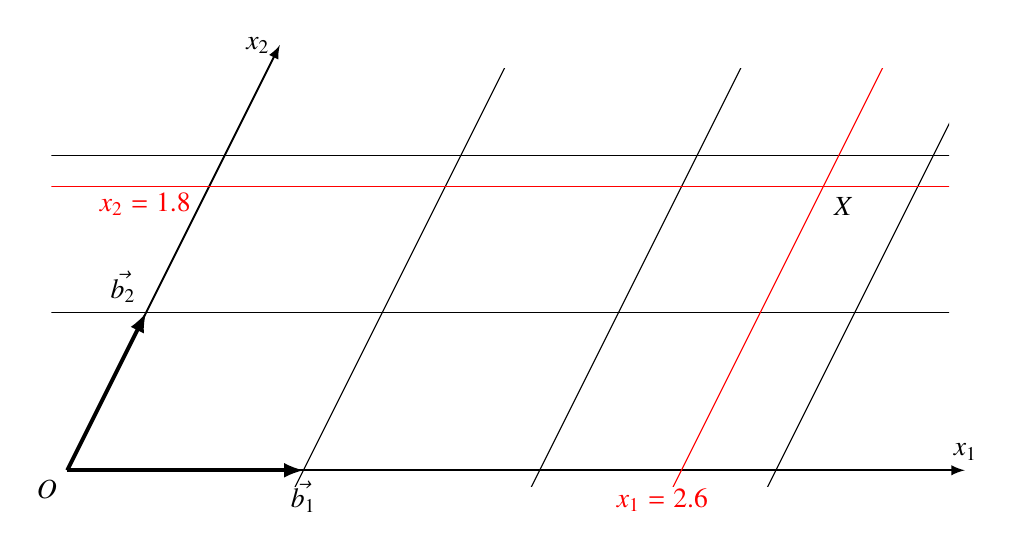
\begin{tikzpicture}[>=latex,thick]

\coordinate (O) at (0,0);
\coordinate (B1) at (3,0);
\coordinate (B2) at (1,2);
\coordinate (X) at ($2.6*(B1)+1.8*(B2)$);


\draw[->,line width=0.7pt] (O) to ($3.8*(B1)$) coordinate[label={above:$x_1$}];
\draw[->,line width=0.7pt] (O) to ($2.7*(B2)$) coordinate[label={left:$x_2$}];

\draw[->,line width=1.4pt] (O)--(B1);
\draw[->,line width=1.4pt] (O)--(B2);

\begin{scope}

\clip (-0.2,-0.2) rectangle (11.2,5.1);

\draw[line width=0.4pt,shorten >= -1cm, shorten <= -1cm]
	($1*(B1)$) to ($1*(B1)+2.2*(B2)$);
\draw[line width=0.4pt,shorten >= -1cm, shorten <= -1cm]
	($2*(B1)$) to ($2*(B1)+2.2*(B2)$);
\draw[line width=0.4pt,shorten >= -1cm, shorten <= -1cm]
	($3*(B1)$) to ($3*(B1)+2.2*(B2)$);

\draw[line width=0.4pt,shorten >= -1cm, shorten <= -1cm]
	($1*(B2)-(B1)$) to ($1*(B2)+3.9*(B1)$);
\draw[line width=0.4pt,shorten >= -1cm, shorten <= -1cm]
	($2*(B2)-(B1)$) to ($2*(B2)+3.9*(B1)$);
\draw[line width=0.4pt,shorten >= -1cm, shorten <= -1cm]
	($3*(B2)-(B1)$) to ($3*(B2)+3.9*(B1)$);

\draw[line width=0.4pt,shorten >= -1cm, shorten <= -1cm,color=red]
	($2.6*(B1)$) to ($(X)+(B2)$);
\draw[line width=0.4pt,shorten >= -1cm, shorten <= -1cm,color=red]
	($1.8*(B2)-(B1)$) to ($(X)+(B1)$);

\end{scope}

\node at (B1) [below] {$\vec{b_1}$};
\node at (B2) [above left] {$\vec{b_2}$};

\punkt{(O)} \node at (O) [below left] {$O$};
\punkt{(X)} \node at (X) [below right] {$X$};

\node[color=red] at ($2.6*(B1)+(-0.25,-0.1)$) [below] {$x_1=2.6$};
\node[color=red] at ($1.8*(B2)+(-0.1,0.05)$) [below left] {$x_2=1.8$};

\end{tikzpicture}

\end{document}

